\documentclass[a4paper]{article}

\usepackage[english]{babel}
\usepackage[utf8]{inputenc}
\usepackage{amsmath}
\usepackage{graphicx}
\usepackage[colorinlistoftodos]{todonotes}

\title{GridPACK Validation Report on State Estimation}

\author{Yousu Chen}

\date{\today}

\begin{document}
\maketitle

This documentation is prepared for validating GridPACK state estimation (SE) function. Because there is not commercial SE tool available to do validation. Therefore, the validation was conducted by two methods: 
\begin{itemize}
  \item Comparing the SE outputs against powerflow solution based measurements. If the maximum absolute difference between SE estimates and measurements is smaller than the tolerance, the SE application meets the validation requirements.  
  \item Comparing against revised Matpower 5.1 SE code. Matpower is a package of MATLAB® M-files for solving power flow and optimal power flow problems that can be downloaded from http://www.pserc.cornell.edu/matpower/.  
\end{itemize}

The details are listed below.

\section{Powerflow based validation}


During the validation, three power systems, 118-bus, 3,000-bus, and 20,000-bus, are used to represent small, medium, and large system. Power flow solutions for each test system are used as measurements. The types of measurements include bus voltage magnitude ($V_M$), real power injection ($P_I$), reactive power injection ($Q_I$), real power flow at both directions ($P_{IJ}$ and $P_{JI}$), reactive power flow at both directions ($Q_{IJ}$ and $Q_{JI}$). Table~\ref{tab:SE}  contains the details of measurement type and associated measurement deviation.

\begin{table} [h]
\centering
\begin{tabular}{l|r}
Type of measurements & Deviation \\\hline
$V_M$	& 0.015 \\
$P_I$	& 0.015 \\
$Q_I$	& 0.015 \\
$P_{IJ}$	& 0.01 \\
$P_{JI}$	& 0.01 \\
$Q_{IJ}$	& 0.01 \\
$Q_{JI}$	& 0.01

\end{tabular}
\caption{\label{tab:SE}Type of measurements and measurement deviations used in State Estimation Validation.}
\end{table}

The SE validation is based on comparing the maximum absolute differences between measurements and SE estimates against SE tolerance. The histogram of these differences for each test systems are provided below.

\subsection{IEEE 118-bus test system}
\label{sec:118}

712 measurements based on power flow solution were applied to the 118-bus test system with a tolerance of $10^{-4}$.  The largest difference between SE output and power flow solution is $6.0*10^{-5}$ which is smaller than the tolerance.  The histogram of the absolute differences between measurements and estimates is shown in Figure  \ref{fig:118}.  Table \ref{tab:118} summaries validation results.

\begin{figure}[ht]
\centering
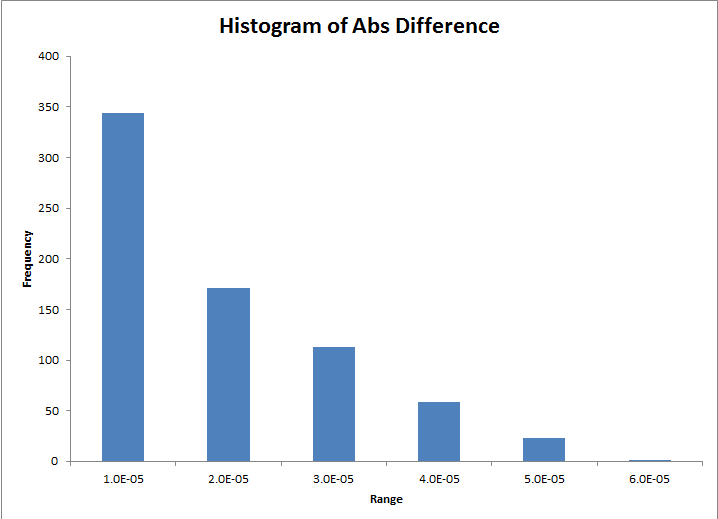
\includegraphics[width=0.8\textwidth]{118.png}
\caption{The histogram of the absolute differences between measurements and estimates for the IEEE 118-bus test system .}
\label{fig:118}
\end{figure}

\begin{table} [h]
\centering
\begin{tabular}{l|r}
Properties & Values \\\hline
The number of measurements & 712 \\
Solution tolerance	& $10^{-4}$ \\
max difference	&  $6.0*10^{-5}$ 
\end{tabular}
\caption{\label{tab:118} Validation results for IEEE 118-bus test system.}
\end{table}


\newpage
\subsection{3000-bus test system}
\label{sec:3000}

For the 3,000-bus system, 24,105 measurements were applied to test the SE. As shown in Figure \ref{fig:3000} , most state estimates are close to the measurements. The largest difference between measurements and estimates is $8.0*10^{-5}$, smaller than the tolerance.  Table \ref{tab:3000} summaries validation results.

\begin{figure}[ht]
\centering
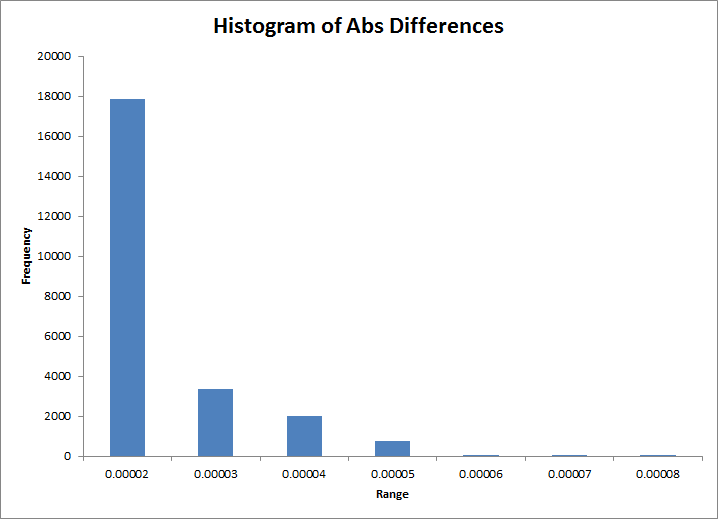
\includegraphics[width=0.8\textwidth]{3000.png}
\caption{The histogram of the absolute differences between measurements and estimates for the 3,000-bus test system .}
\label{fig:3000}
\end{figure}

\begin{table} [h]
\centering
\begin{tabular}{l|r}
Properties & Values \\\hline
The number of measurements & 24,105\\
Solution tolerance	& $10^{-4}$ \\
max difference	&  $8.0*10^{-5}$ 
\end{tabular}
\caption{\label{tab:3000} Validation results for the 3000-bus test system.}
\end{table}

\subsection{20,000-bus test system}
\label{sec:20000}

The 20,000-bus system represents a western United State power grid (WECC system). The number of measurements is 74,747. As shown in Figure \ref{fig:20000}, the largest absolute difference between measurements and estimates is $9.0*10^{-5}$, smaller than the tolerance. Table \ref{tab:20000} summaries validation results.

\begin{figure}[ht]
\centering
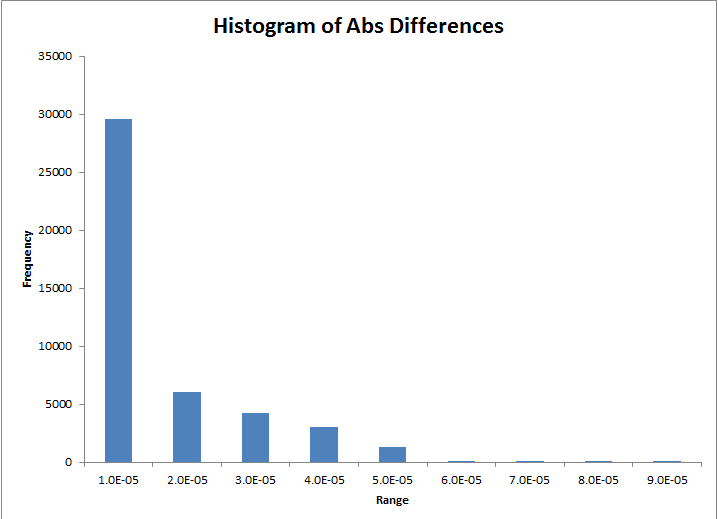
\includegraphics[width=0.8\textwidth]{20000.png}
\caption{The histogram of the absolute differences between measurements and estimates for the 20,000-bus test system.}
\label{fig:20000}
\end{figure}

\begin{table} [h]
\centering
\begin{tabular}{l|r}
Properties & Values \\\hline
The number of measurements & 74,747 \\
Solution tolerance	& $10^{-2}$ \\
max difference	&  $9.0*10^{-5}$ 
\end{tabular}
\caption{\label{tab:20000} Validation results for  the 20,000-bus test system.}
\end{table}

\section{Matpower based validation}

Matpower version 5.1 has a state estimation (SE) package that is used to do validation. The fundamental SE algorithm algorithm is the same as the one in GridPACK, with following minor differences.

\begin{enumerate}
  \item In Matpower, the measurements at reference bus are known. 
  \item The power injection measurements used in Matpower are the generation outputs, instead of net injections.
\end{enumerate}
To have a fair comparison between GridPACK and Matpower, following changes are made.
\begin{enumerate}
  \item In Matpower, change the Sgen variable at doSE.m to net injection at generator bus. (Sgen = Sgbus) 
  \item In Matpower, modify the measurements in generator buses to net injections. (substract corresponding load value at each bus)
  \item In GridPACK, add a Vm measurement at the reference bus with a small weight (0.0000001) to make it "known" as Matpower does.
\end{enumerate}

Matpower has a test file set up with the IEEE 14-bus system. The same test case is used to validate GridPACK SE function. The simulation results from GridPACK and Matpower are listed in Table \ref{tab:GridPACKSEBus}, \ref{tab:GridPACKSEBranch}, and \ref{tab:MatpowerSE}. These simulation results show that GridPACK and Matpower match pretty well. Please note that $IJ$ and $JI$ in GridPACK measurements corresponds to $F$ and $T$ in Matpower measurements

\begin{table} [ht]
\centering
\begin{tabular} {c|c|c|c|c}
	\hline
  Type  &  Bus Number &    Measurement &         Estimate &        Difference \\
     PI  &      1     &        2.32000 &          2.32458 &           0.00458 \\
     QI  &      1     &       -0.16900 &         -0.13831 &           0.03069 \\
     VM  &      1     &        1.06000 &          1.06000 &          -0.00000 \\
     PI  &      2     &        0.18300 &          0.18480 &           0.00180 \\
     QI  &      2     &        0.29700 &          0.30806 &           0.01106 \\
     VM  &      2     &        1.00000 &          1.04385 &           0.04385 \\   
     PI  &      3     &       -0.94200 &         -0.94198 &           0.00002 \\     
     VM  &      3     &        1.00000 &          1.00700 &           0.00700 \\     
     PI  &      6     &       -0.11200 &         -0.11105 &           0.00095 \\     
     VM  &      6     &        1.00000 &          1.11981 &           0.11981 \\     
     PI  &      8     &        0.00000 &         -0.00000 &          -0.00000 \\     
     VM  &      8     &        1.00000 &          1.00000 &          -0.00000 \\     
     VM  &     10     &        1.00000 &          1.00000 &           0.00000 \\     
     VM  &     14     &        1.00000 &          1.00000 &           0.00000 \\
     \hline
\end{tabular}
\caption{GridPACK SE results of IEEE 14-bus System for bus values} \label{tab:GridPACKSEBus} 
\end{table}


\begin{table} [ht]
\centering
\begin{tabular} {c|c|c|c|c|c|c}
\hline
    Type & From& To & CKT & Measurement & Estimate &   Difference \\
    PIJ  &  1  &  2 &  BL &   1.57080 &   1.56751 &      -0.00329 \\
    QIJ  &  1  &  2 &  BL &  -0.17480 &  -0.18359 &      -0.00879 \\
    PIJ  &  2  &  3 &  BL &   0.73400 &   0.73141 &      -0.00259 \\
    QIJ  &  2  &  3 &  BL &   0.05940 &   0.04517 &      -0.01423 \\
    PJI  &  2  &  4 &  BL &  -0.54270 &  -0.54308 &      -0.00038 \\
    QJI  &  2  &  4 &  BL &   0.02130 &   0.02041 &      -0.00089 \\
    PJI  &  2  &  5 &  BL &  -0.40810 &  -0.40912 &      -0.00102 \\
    QJI  &  2  &  5 &  BL &  -0.01930 &  -0.02149 &      -0.00219 \\
    PJI  &  4  &  5 &  BL &   0.60060 &   0.59949 &      -0.00111 \\
    QJI  &  4  &  5 &  BL &  -0.10060 &  -0.10554 &      -0.00494 \\
    PIJ  &  4  &  7 &  BL &   0.27070 &   0.27091 &       0.00021 \\
    QIJ  &  4  &  7 &  BL &  -0.15400 &  -0.15965 &      -0.00565 \\      
    PIJ  &  4  &  9 &  BL &   0.15460 &   0.15366 &      -0.00094 \\    
    QIJ  &  4  &  9 &  BL &  -0.02640 &  -0.01173 &       0.01467 \\ 
    PIJ  &  5  &  6 &  BL &   0.45890 &   0.45033 &      -0.00857 \\
    QIJ  &  5  &  6 &  BL &  -0.20840 &  -0.09830 &       0.11010 \\
    PJI  &  6  &  11&  BL &  -0.08160 &  -0.07989 &       0.00171 \\
    QJI  &  6  &  11&  BL &  -0.08640 &  -0.08638 &       0.00002 \\
    PIJ  &  6  &  13&  BL &   0.18340 &   0.18084 &      -0.00256 \\
    QIJ  &  6  &  13&  BL &   0.09980 &   0.09982 &       0.00002 \\
    PIJ  &  7  &  9 &  BL &   0.27070 &   0.27074 &       0.00004 \\
    QIJ  &  7  &  9 &  BL &   0.14800 &   0.14516 &      -0.00284 \\
    PIJ  &  9  &  10&  BL &   0.05230 &   0.05230 &      -0.00000 \\
    PIJ  &  9  &  14&  BL &   0.09430 &   0.09430 &      -0.00000 \\
    PIJ  &  12 &  13&  BL &   0.01880 &   0.02045 &       0.00165 \\
\hline
\end{tabular}
\caption{GridPACK SE results of IEEE 14-bus system for branch values} \label{tab:GridPACKSEBranch} 
\end{table}


\begin{table} [ht]
\centering
\begin{tabular} {c|c|c|c}
\hline
    Type    &    Index &    Measurement &  Estimation \\
      PF    &      1   &       1.5708   &      1.5675 \\
      PF    &      3   &       0.7340   &      0.7314 \\
      PF    &      8   &       0.2707   &      0.2709 \\
      PF    &      9   &       0.1546   &      0.1537 \\
      PF    &     10   &       0.4589   &      0.4503 \\
      PF    &     13   &       0.1834   &      0.1808 \\
      PF    &     15   &       0.2707   &      0.2707 \\
      PF    &     16   &       0.0523   &      0.0523 \\
      PF    &     17   &       0.0943   &      0.0943 \\
      PF    &     19   &       0.0188   &      0.0205 \\
      PT    &      4   &      -0.5427   &     -0.5431 \\
      PT    &      5   &      -0.4081   &     -0.4091 \\
      PT    &      7   &       0.6006   &      0.5995 \\
      PT    &     11   &      -0.0816   &     -0.0799 \\
      PG    &      1   &       2.3200   &      2.3246 \\
      PG    &      2   &       0.1830   &      0.1848 \\
      PG    &      3   &      -0.9420   &     -0.9420 \\
      PG    &      4   &      -0.1120   &     -0.1111 \\
      PG    &      5   &       0.0000   &      0.0000 \\
      QF    &      1   &      -0.1748   &     -0.1836 \\
      QF    &      3   &       0.0594   &      0.0452 \\
      QF    &      8   &      -0.1540   &     -0.1596 \\
      QF    &      9   &      -0.0264   &     -0.0117 \\
      QF    &     10   &      -0.2084   &     -0.0983 \\
      QF    &     13   &       0.0998   &      0.0998 \\
      QF    &     15   &       0.1480   &      0.1452 \\
      QF    &     19   &       0.0141   &      0.0134 \\
      QT    &      4   &       0.0213   &      0.0204 \\
      QT    &      5   &      -0.0193   &     -0.0215 \\
      QT    &      7   &      -0.1006   &     -0.1055 \\
      QT    &     11   &      -0.0864   &     -0.0864 \\
      QG   &       1   &      -0.1690   &     -0.1383 \\
      QG   &       2   &       0.2970   &      0.3081 \\
      Vm   &       2   &       1.0000   &      1.0438 \\
      Vm   &       3   &       1.0000   &      1.0070 \\
      Vm   &       6   &       1.0000   &      1.1198 \\
      Vm   &       8   &       1.0000   &      1.0000 \\
      Vm   &      10   &       1.0000   &      1.0000 \\
      Vm   &      14   &       1.0000   &      1.0000 \\
\hline
\end{tabular}
\caption{Matpower SE results for the IEEE 14-bus system} \label{tab:MatpowerSE} 
\end{table}

\bigskip
In summary, all the test results above have shown that GridPACK SE meets the validation requirements.

\end{document}